\label{sec:relatedworks}
\subsection{Генеративные состязательные сети}
% https://arxiv.org/pdf/2004.02546.pdf -- see Background for decent architecture explanation... 

Генеративные состязательные сети (\emph{Generative adversarial network}, сокр., \emph{GAN})  это семейство генеративных моделей, разработанное Яном Гудфеллоу в 2014 году \cite{goodfellow2014generative}.  Они формулируют процесс обучения  генеративной модели в виде антагонистической игры между двумя игроками: \emph{генератором} и \emph{дискриминатором}.

Генератор $G$ представляет собой глубокую нейронную сеть, задающую отбражение из латентного пространства $Z$ в пространство данных $\mathcal X$.
Принимая на вход случайные вектора из некоторого заданного распределения $p(z)$ в $Z$, он производит набор синтетических данных, пытаясь аппроксимировать распределение обучающей выборки $q_{data}(x)$.

Дискриминатор $D$ представляет собой глубокую нейронную сеть, задающую отбражение из пространства данных $\mathcal X$ в $\mathbb R$. Получив на вход некоторый элемент из пространства $\mathcal X$, дискриминатор ~возвращает~(характеризует) вероятность того, что он был получен из распределения реальных данных $q_{data}(x)$, а не сгенерирован генератором $G$.

\begin{figure}[h]
\begin{center}
    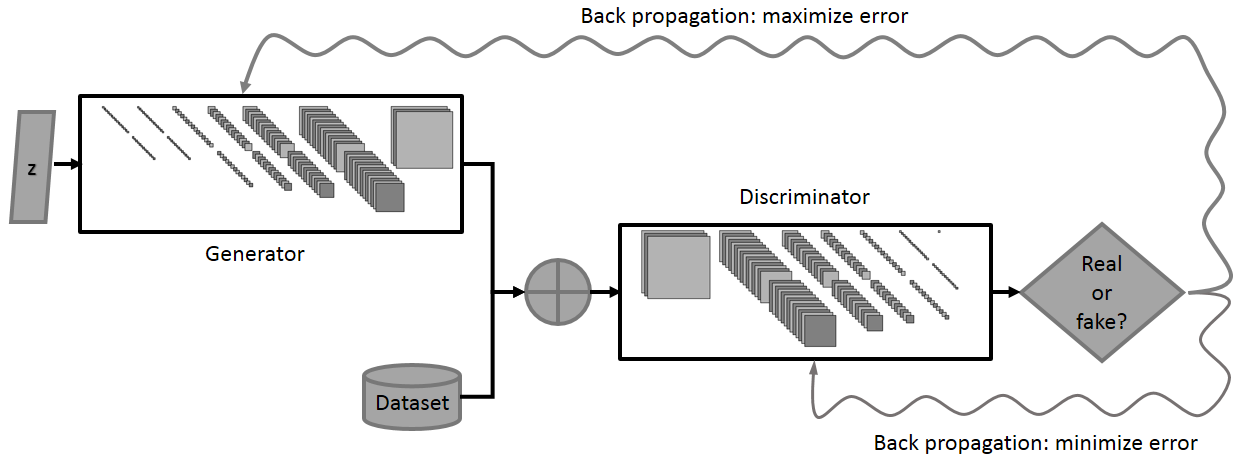
\includegraphics[width=0.9\textwidth]{gan}
    \caption{Архитектура генеративной состязательной сети (написать откуда взял)}
    \label{fig:subim11}
\end{center}
\end{figure}

Роль дискриминатора состоит в том, чтобы как можно более точно отличать синтетические данные, полученные генератором, от реальных данный, взятых из обучающей выборки, в то время как генератор пытается обмануть дискриминатор путем генерирования синтетических данных, как можно более похожих на реальные.
Процесс совместного конкурентного обучения продолжается вплоть до достижения парой $(G, D)$ <<седловой точки>> (т.е. равновесия по Нэшу) \cite{goodfellow2017nips} функции выигрыша
$$
\min_{G} \max_{D} V(G, D) = \mathop{\mathbb{E}}_{x \sim q_{data}(x)} [\log D(x)] + \mathop{\mathbb{E}}_{z \sim p(z)} [\log (1 - D(G(z)))] ,
$$
в которой генератор способен генерировать данные, неотличимые дискриминатором от реальных.

\subsection{Генеративные нейронные сети для генерации лиц}

При решении задачи генерации изображений (в.т.ч. изображений лиц), в качестве дискриминатора используется сверточная нейронная сеть [VGG / conv ?], а в качестве генератора --- сверточная нейронная сеть со слоями транспонированной свертки [DCGAN].
Пространство данных $\mathcal X$ в данном случае предстваляет собой пространство изображений, каждый элемент которого обладает некоторым набором семантических признаков, например в случае лиц --- положение головы, пол, возраст.

\paragraph{BigGAN.}
Генерация изображений высокого разрешения довольно долго была трудной(непосильной) задачей для GAN-ов. Она требует генеративной модели с большим количеством параметров, что, в случае GAN-ов, сказывается на стабильности обучения [че то типа Why GANs are hard to train].

% ... разработанная компанией DeepMind.
(Генеративная состязательная сеть) BigGAN \cite{bigGAN} являлась ?первым шагом к решению данной проблемы. Эта сеть спроектирована с целью масштабирования архитектуры для генерации изображений высокого разрешения.
Она внесла ряд модификаций в стандартную архитектуру генеративных состязательных сетей (и процесс генерации), таких как self-attention слой, спектральная нормализация весов (, Truncation Trick). Это позволило увеличить количество весов модели в 2 раза и добиться качественной генерации изображений с разрешением до $512\times512$ на самых разнообразных классах изображений.


\paragraph{StyleGAN.}
StyleGAN \cite{StyleGAN} – это генеративная состязательная сеть, архитектура которой разрабатывалась специально с целью генерации реалистичных изображений лиц.
Одной из сложностей генерации изображений является кривизна, или запутaнность (\emph{entanglement}), латентного пространства. 
Входное латентное пространство $\mathcal Z$ должно подстраиваться под вероятносное распределение тренировочных данных, а потому любые сдвиги/неточности, например отсутствие в тренировочных данных комбинации нескольких признаков (Рис. \ref{fig:stylegan-mapping}), приводят к искажениям.
В результате латентное пространство (приходится рассматривать) не как линейное евклидово пространство, а как искривленное пространство \cite{arvanitidis2018oddity}.

% Для решения этой проблемы...
Одной из ключевых особенностей архитекуры StyleGAN является наличие промежуточного латентного пространства $\mathcal W$. Во время обучения StyleGAN выучивает нелинейное преобразование $f: \mathcal Z \mapsto \mathcal W$, что позволяет избавиться от ограничений, накладываемых вероятносным распределением тренировочных данных, и получить более линейное латентное пространство.

% реализует архитектуру ...?
StyleGAN предлагает альтернативную архитектуру генератора, которая основывается на идеях из style transfer. 
Синтез изображения начинается с фиксированного входного вектора, а информация о латентном представлениии последовательно встраивается в каждый слой генератора, начиная с первых слоев генератора с пространственной размерностью $4\times4$ и заканчивая последними слоями с размерностью $1024\times1024$.
Это позволяет контролировать силу проявления различных семантических признаков изображения на разных ?масштабах, от грубых признаков до тонких деталей.
В сочитании с встраивании шума напрямую в слои сети, такая архитектура позволяет отделить высокоуровневые атрибуты изображения (положения лица, личность человека) от случайных вариационных факторов (волосы, веснушки и т.п.).

\begin{figure}[h]
\begin{center}
    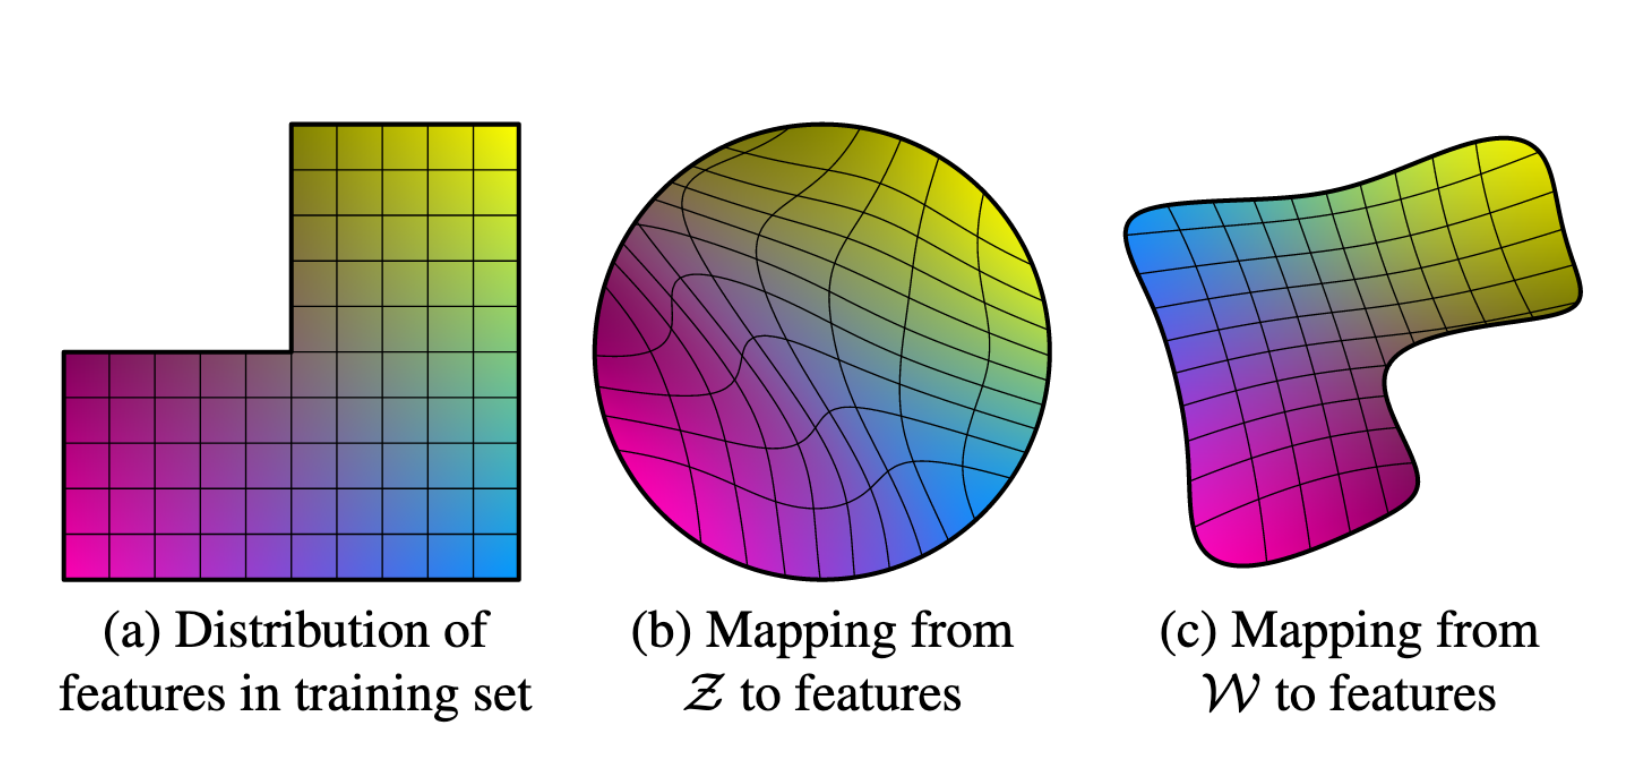
\includegraphics[width=0.7\textwidth]{stylegan_mapping}
    \caption{Иллюстрация действия промежуточного латентного пространства на примере двух факторов вариации. Изображение взято из \cite{StyleGAN}. \emph{Расписать a, b, c.}}
    \label{fig:stylegan-mapping}
\end{center}
\end{figure}
% Illustrative example with two factors of variation (image features, e.g., masculinity and hair length).  (a) An example training set where some combination (e.g., long haired males) is missing. (b) This forces the mapping from Z to image features to become curved so that the forbidden combination disappears in Z to prevent the sampling of invalid combinations.  (c) The learned mapping from Z to W is able to “undo” much of the warping.


\paragraph{ALAE.}
% We designed an AE architecture where we allow the latent distribution to be learned from data to address entanglement (A). The output data distribution is learned with an adversarial strategy (B). Finally, to implement (A) and (B) we impose the AE reciprocity in the latent space (C).

% декомпозируем генератор и дискриминатор ... - но это не очень понятно
ALAE \cite{ALAE} – это генеративная нейронная сеть, которая совмещает в себе особенности генеративных состязательных сетей и вариационных автоэнкодеров [].

Она модифицирует стандартную архитектуру генеративных состязательных сетей путем добавления \emph{перед} генератором и \emph{перед} дискриминатором некоторых выучваемых отображений в промежуточное латентное пространство.
% наложение на промежуточное латентное пространство ограничения о взаимной близости представлений дает возможность выучить latent distribution с помощъю autoencoder стратегии, и data distribution с помощью состязательной стратегии.
Из-за этого он жертвует качеством генерации, но дополнительно выучивает обратное отображение в латентное пространство сети.


\subsection{Алгоритмы отображения изображений в латентное пространство сети}
% TODO выровнять алгоритмы/методы/подходы
Для работы с реальными изображениями генеративным состязательным сетям требуется обратное отображение, позволяющее по входному изображению получить соответствующий ему латентный вектор. 
Классическая архитектура генеративных состязательных сетей не задает такого отображения напрямую, а потому для работы с реальными изображениями реализуются алгоритмы, позволяющие аппроксимировать данный латентный вектор.

%% \subsubsection{Обучение дополнительного энкодера}
Одним из самых распространенных является обучение энкодера \cite{donahue2016adversarial} --- дополнительной нейронной сети, которая будет отображать входное изображение в латентное пространство заданной генеративной состязательной сети.
% датасет --> набор данных
Энкодер имеет сверточную архитектуру, и процесс его обучения сводится к задаче регрессии латентного вектора по заданному входному изображению. 
Обучение энкодера производится на датасете пар <\emph{изображение, вектор}>, состоящем из набора синтетических изображений, сгенерированных генеративной состязательной сетью, и входных векторов, с помощью которых изображение было получено.

%% \subsubsection{Латентная оптимизация}
Латентная оптимизация \cite{perarnau2016invertible} --- это алгоритм приближения латентного вектора, который заключается в нахождении латентного вектора путем минимизации некоторой заданной функции потерь реконструкции.
% Этот алгоритм задает функцию потерь $ f(x_real, G(z)) $, которая показывает, насколько сгенерированное изображение близко к входному.
% Примером такой функции потерь может служить среднеквадратичная ошибка в пространстве пикселей (pixel-wise), или perpetual loss, заданный в пространстве признаков, извлеченных сетью VGG[]. 
% https://arxiv.org/abs/2002.04185 -- Smoothness and Stability in GANs
% Кратко описать условия, при которых GD сойдется
% Under the assumption of generator being smooth (which, since generator is a composition of linear maps and activation functions, depends only on smoothness of activations), we can use gradient descent to minimize reconstruction loss.
% Поскольку генератор является отображением, дискпвтпоп по входному вектору, а его гладкость зависит главным образом от гладкости функций активации [], это позволяет минимизировать ф.п. с помощью г.с., итеративно обновляя латентный вектор.
Генератор сети GAN является композицией линейных слоев и функций активации, а потому при использовании гладких функций активации также является гладким отображением.
Это позволяет применить градиентный спуск и метод обратного распространения ошибки для нахождения латентного вектора, минимизирующего заданную функцию потерь реконструкции.

% Использование арзитектуры StyleGAN позволяет еще больше улучшить процесс латентной оптимизации. Оптимизация в промежуточном латентном пространства W, в меньшей степени подверженного искривлению, позволяет стабилизировать градиентный спуск [Image2StyleGAN ?]. Кроме того, архитектура StyleGAN устроена таким образом, что вместо последовательных перобразований над латентным вектором, латентный вектор подается на вход каждому слою генератора in parallel fashion. Это позволяет латентный вектор каждого латентного слоя оптимизировать отдельно, тем самым получив оптимизацию в раширенном промежуточном пространстве W+. В результате такой оптимизации можно получить изображения, которые невозможно было бы сгенерировать в стандартном pipeline. [What GANs cannot generate, Cheese theorem].


\subsection{Алгоритмы выделения семантик изображения в латентном пространстве сети}
Идея манипулирования латентным вектором в латентном пространстве генеративной состязательной сети основана на наблюдении о том, что к латентным векторам применима векторная арифметика \cite{radford2015unsupervised}.
% Из этого возникает идея нахождения преобразований в латентном пространстве, которые соответствовали бы изменениям семантических признаков на генерируемом изображениии.
% Большинство (?) исследований (св-в латентного пространства) основываются на пердположении о линейности латентного пр-ва / о том, что отдельным факторам вариации генерируемых изображений (изображений из тренировочной выборки) соответствует некоторое линейное подпространство в латентном пр-ва.
% Линейный сдвиг в направлении ...
% (Нужно конкретно определить, что мы ищем, т.е. important directions / semantics -- найти для этого русское определение).

% Далее говорим про GANSpace, котороый использует метод главных компонент для выделения значимых направлений. Требуется дальнейший визуальный анализ, чтобы определить, каким изменениям/семантикам они соответствуют.
Другой подход \cite{hrknen2020ganspace} использует метод главных компонент для уменьшения размерности латентного пространства и выделения наиболее важных направлений. Дальнейший визуальный/качественный анализ полученных направлений показывает, что они соответствуют значимым изменениям в изображении.

% Для более качественного исследования ?направлений? в латентном пространстве InterFaceGAN предлагает находить направления путем нахождения/фиттинга оптимальной разделяющей гиперплоскости. 
Один из существующих подходов \cite{shen2020interfacegan} выдвигает предположение о линейности латентного пространства, и исследует его с целью нахождения векторов, соответствующих определенным заданным изменениям в признаках изображения.
